% THIS IS SIGPROC-SP.TEX - VERSION 3.0
% WORKS WITH V3.1SP OF ACM_PROC_ARTICLE-SP.CLS
% JUNE 2007
%
% It is an example file showing how to use the 'acm_proc_article-sp.cls' V3.1SP
% LaTeX2e document class file for Conference Proceedings submissions.
% ----------------------------------------------------------------------------------------------------------------
% This .tex file (and associated .cls V3.1SP) *DOES NOT* produce:
%       1) The Permission Statement
%       2) The Conference (location) Info information
%       3) The Copyright Line with ACM data
%       4) Page numbering
% ---------------------------------------------------------------------------------------------------------------
% It is an example which *does* use the .bib file (from which the .bbl file
% is produced).
% REMEMBER HOWEVER: After having produced the .bbl file,
% and prior to final submission,
% you need to 'insert'  your .bbl file into your source .tex file so as to provide
% ONE 'self-contained' source file.
%
% Questions regarding SIGS should be sent to
% Adrienne Griscti ---> griscti@acm.org
%
% Questions/suggestions regarding the guidelines, .tex and .cls files, etc. to
% Gerald Murray ---> murray@acm.org
%
% For tracking purposes - this is V3.0SP - JUNE 2007

\documentclass{acm_proc_article-sp}

\begin{document}

\title{On the Benefits of Scenario Variability as Crosscutting}

%
% You need the command \numberofauthors to handle the 'placement
% and alignment' of the authors beneath the title.
%
% For aesthetic reasons, we recommend 'three authors at a time'
% i.e. three 'name/affiliation blocks' be placed beneath the title.
%
% NOTE: You are NOT restricted in how many 'rows' of
% "name/affiliations" may appear. We just ask that you restrict
% the number of 'columns' to three.
%
% Because of the available 'opening page real-estate'
% we ask you to refrain from putting more than six authors
% (two rows with three columns) beneath the article title.
% More than six makes the first-page appear very cluttered indeed.
%
% Use the \alignauthor commands to handle the names
% and affiliations for an 'aesthetic maximum' of six authors.
% Add names, affiliations, addresses for
% the seventh etc. author(s) as the argument for the
% \additionalauthors command.
% These 'additional authors' will be output/set for you
% without further effort on your part as the last section in
% the body of your article BEFORE References or any Appendices.

\numberofauthors{3} %  in this sample file, there are a *total*
% of EIGHT authors. SIX appear on the 'first-page' (for formatting
% reasons) and the remaining two appear in the \additionalauthors section.
%
\author{
\alignauthor
Rodrigo Bonif\'{a}cio\\
       \affaddr{Informatics Center}\\
       \affaddr{Federal University of Pernambuco}\\
       \affaddr{Recife, Brazil}\\
       \email{rba2@cin.ufpe.br}
\alignauthor
Paulo Borba\\
       \affaddr{Informatics Center}\\
       \affaddr{Federal University of Pernambuco}\\
       \affaddr{Recife, Brazil}\\
       \email{phmb@cin.ufpe.br}
\alignauthor
S\'{e}rgio Soares\\
       \affaddr{Department of Computing and Systems}\\
       \affaddr{University of Pernambuco}\\
       \affaddr{Recife, Brazil}\\
       \email{sergio@dsc.upe.br}
}
\maketitle

\begin{abstract}
Variability management allows product customization by specifying
variation points and composition rules related to feature models and
product configurations. This is an interesting kind of crosscutting
concern, since a feature might require variation points to be spread
into different artifacts of each Software Product Line model
(requirements, design, source code, and tests). In order to modularize
use case
scenario variability management, we proposed a crosscutting approach
that weaves scenarios, feature models, product configurations, and
configuration knowledge. The result leads to independent specification
of behavior and variability concerns. In this work, we report the
benefits of such kind of \emph{separation of concerns} by comparing our
approach with other techniques for handling scenario variability
management. 
%This comparison was based on Design
%Structure Matrixes (DSMs), on modularity and complexity metrics, and
%on response to evolution for common increments in a real product line.
\end{abstract}


\category{D.2.1}{Software Engineering}{Requirements}[Languages,
Methodologies]\
\category{D.2.13}{Software Engineering}{Reusable
Software}

\terms{Design, Documentation}

\keywords{Software product line, variability management, requirement models}

\section{Introduction}
The Software Product Line (SPL) approach for software development corresponds to a set of practices that allows strategic reuse by observing commonalities among applications in a shared domain~\cite{northrop-spl-book,phol-spl-book}. Based on specific feature configurations, each member of the product line is assembled by selecting, creating, or customizing specific artifacts. In this way, features, that describe the SPL variability space, must be related to variation points that allows product customization. 
Identifying what are the variation points required for each feature, which techniques are suitable for specifying them, and how they should be related to feature models are the main goals of variability management concern. Actually, this is an interesting kind of crosscutting concern, since features might require variation points to be spread into different artifacts of SPL models. 

Specifically in the context of requirement artifacts, several techniques for use case scenario variability management were proposed~\cite{favaro-icsr-98,bertolino-esec-2003,fantechi-splc-2004,eriksson-splc-2005}. However, existing works are basically concerned about how to represent variation points in scenario specification; but critical properties of variability management, such as scalability upon common SPL increments and high degrees of specification reuse, are not well addressed. We argue that, due to the crosscutting characteristic of variability management, it is necessary to create a clear separation between scenario specification and variability management. Our approach (Section~\ref{scenario-variability}) weaves several specifications (feature model, product configuration, configuration knowledge, and use case model), which crosscut each other, to better modularize scenario variability management. 

In this paper, we report the benefits of our approach to support common increments in a real SPL (introduced in Section~\ref{mms-pl}). We achieve such goal by comparing our approach to PLUC~\cite{bertolino-esec-2003} and PLUSS~\cite{eriksson-splc-2005}, two representative notations for SPL scenario variability. In order to increase our confidence, different modularity analysis techniques were used: Design Structure Matrices (Section~\ref{dsm-analysis}), a suite of metrics (Section~\ref{quantitative-analysis}), and observations of the effort needed to introduce SPL increments using each approach (Section~\ref{evolution-analysis}). The main contributions of this paper are

\begin{itemize}
\item A comparative analysis that suggests the need for a better separation between variability management and SPL artifacts. Although our evaluation is restricted to use case scenario artifacts, we believe that such separation is also useful for other product line artifacts, and has already been claimed for source code~\cite{alves-gpce-06,mmedeiros-lawasp-2007}.

\item An approach for comparing variability management techniques. This approach is based on techniques and common SPL increments that can also be applied to analyze modularity in other SPL artifacts. Actually, similar techniques have being used to evaluate modularity in source code~\cite{vlopes-aosd-2005, sullivan-fse-2005,garcia-taosd-2005, greenwood-ecoop-2007}.   

\end{itemize}

Finally, we compare our approach to the body of related work (Section \ref{related-work}) and present our concluding remarks in 
Section~\ref{concluding-remarks}. Next, we introduce our approach for scenario variability management.
   
\section{Variability as Crosscutting}
\label{scenario-variability}

Variability management, as discussed in the previous section, is well known as a crosscutting concern. Therefore, in order to increase modularity, it is necessary to provide a clear separation between 
variability management and typical software development assets (such as requirements, design, source code, and test cases). The result is that both representations can then evolve independently. However, such kind of separation of concerns (SoC) also requires mechanisms to weave these representations during the product engineering phase~\cite{northrop-spl-book}.

We proposed a modeling framework for use case scenario variability that takes into account the crosscutting nature of variability management. Applying the modeling framework, we described a \emph{weaver} that takes four specifications as input (\emph{product line use case model}, \emph{feature model}, \emph{product configuration}, and \emph{configuration knowledge}) that crosscut each other with respect to the resulting product specific use case model (Figure~\ref{fig:wp}). This weaver presents a clear separation between variability management and scenario specification, and also describes the 
processes required to compose those input specifications. 

\begin{figure}[h]
\centering
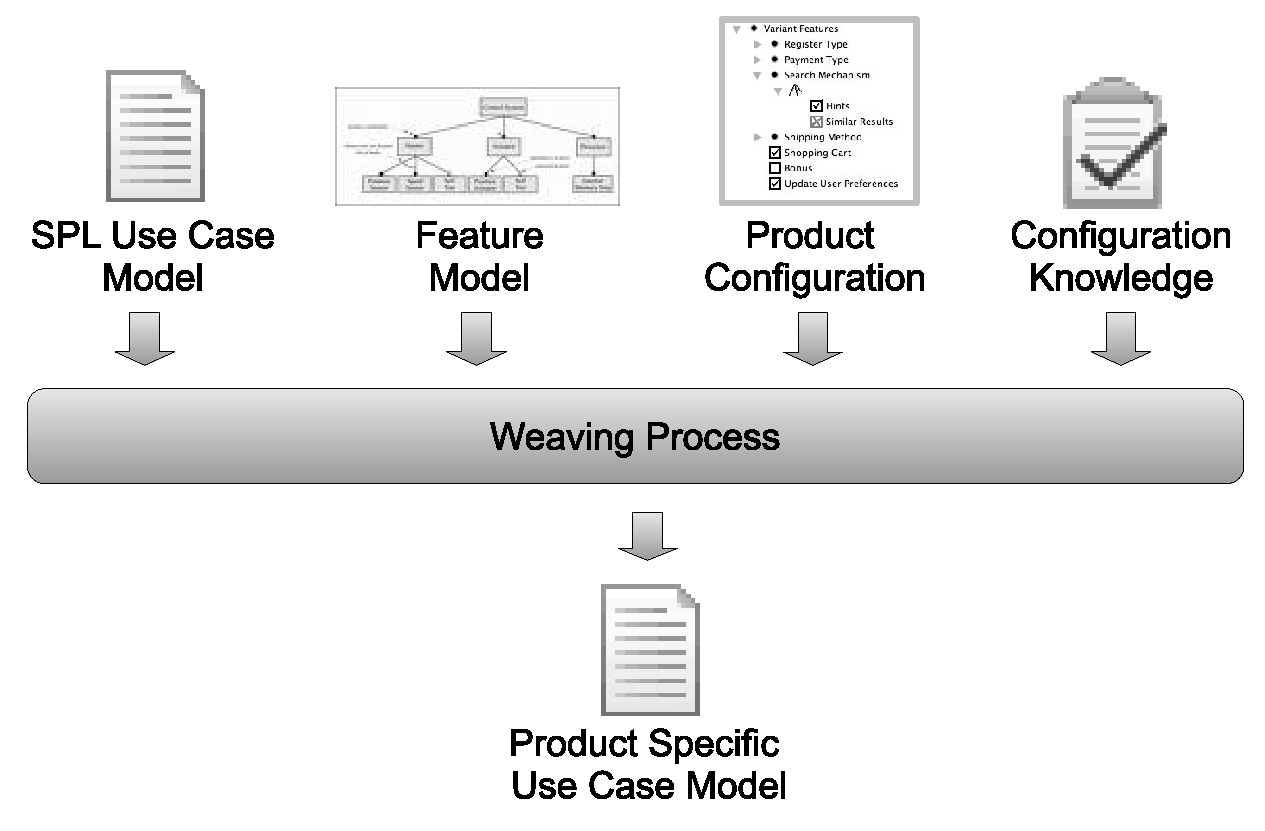
\epsfig{file=images/weave-process.eps,scale=0.35}
\caption{Overview of the weaving process}
\label{fig:wp}
\end{figure}

It is interesting to enforce that such composition allows the representation of different kinds of variability, such as \emph{optional use cases and scenarios}, \emph{quantified changed scenarios}, and 
\emph{parameterized scenarios}. The weaver was decomposed in subprocesses\footnote{Actually, each subprocess is also a weaver represented in our modeling framework.}, one for each kind of variability. The semantics of those weavers (and the meta-model of the input and output languages) were described using the Haskell programming language~\cite{haskell-report}.

The first weaver is responsible for checking if a product configuration is a valid instance of the feature model and for selecting, based on the product configuration, the set of use cases and scenarios that should be assembled into the final product. The second weaver, instead, is responsible for composing the resulting scenarios of first weaver, since they might crosscut each other based on \emph{from steps} and \emph{to steps} clauses (Figure~\ref{fig:cc-01}). These clauses are used to modularize specifications, in such way that one scenario can crosscut scenarios of different use cases. For instance, Figure~\ref{fig:cc-01} depicts that the behavior of \emph{Insert a DRM restricted content in warning mode} crosscuts the behavior of \emph{Include a multimedia content} after step \emph{A1.1} and then returns to step \emph{4M} of \emph{Create and send a multimedia message}.  As a consequence, after weaving the scenarios showed in Figure~\ref{fig:cc-01}, the following sequence of events is valid:

\begin{center}
\small{
\fbox{$<1M, 2M, 3M, A1.1, CM.1, CM.2, 4M, 5M, 6M>$}
}
\end{center}

Finally, the third weaver is responsible for binding parameters embedded in scenario specifications. For example, the \emph{Include a multimedia content} scenario in Figure~\ref{fig:cc-01} is parameterized according to the content types supported by a specific product. The domain values of parameters are defined in the product configuration. Therefore, if a product is configured with supporting for image and audio content types, only these options will be available.  In order to reduce coupling, a separated mapping is used for relating parameters embedded in scenarios to features selected in specific configurations. This decision preserves the independence between these artifacts.

\begin{figure}[h]
\begin{center}
\begin{tiny}
  \texttt{
  \begin{tabular}{l}
  {\bf Use Case: Create and Send a Message}  \\ Id: 01 \\
  {\bf Goal: Create and send a multimedia message}  \\
  {\bf Main Flow:  The message box is not full.} \\ 
  {\bf From step: START} \\
  {\bf To step: END} \\
  \end{tabular}
  \begin{tabular}{|p{0.2in}|p{1in}|p{0.8in}|p{1in}|}
  \hline 
  id & User Action & System State & System Response \\ \hline 
  1M  & Starts the message center application & & The message center application is started \\ \hline
  2M  & Selects Create New MMS option & &The create a new MMS form is displayed \\ \hline
  3M  & Fills in the message body & & The message body is filled in \\ \hline
  4M &  Selects the send message option &  & The recipient form is displayed \\ \hline
  5M  & Fills in the recipient field & & The recipient field is filled \\ \hline
  6M  & Selects the confirm option & The message has not reached <FolderSize> messages & The message is sent to the recipient and saved in the sent folder. The application returns to message center \\ \hline
 \end{tabular}
 %First extension flow in PLUSS example 
 \begin{tabular}{l}
  \\
 {\bf Alternative Flow:  Include a multimedia content} \\ 
 {\bf From step: 3M,4M} \\
  {\bf To step: 4M} \\
 \end{tabular}
   \begin{tabular}{|p{0.2in}|p{1in}|p{0.8in}|p{1in}|}
  \hline  
   id & User Action & System State & System Response \\ \hline 
  A1.1  & Select the include a <ContentType> option & &The list of all <ContentType> available content type is displayed \\ \hline
  A1.2 & Selects a specific resource & &  The selected resource is attached to the multimedia message   \\ \hline
  \end{tabular} 
 %Second extension flow in PLUSS example  
  \begin{tabular}{l} 
     \\
    Other alternative scenarios should be specified here \\ \\
  \end{tabular}
  \begin{tabular}{l}
  {\bf Use Case: Composition Mode Related to DRM Restrictions}  \\ Id: 02 \\ 
  {\bf Goal: Changes the composition behavior depended on DRM configuration}   \\
  {\bf Alternative Flow:  Insert a DRM restricted content in warning mode} \\ 
  {\bf From step: UC01/A1.1 }\\
  {\bf To step: UC01/4M} \\
  \end{tabular}
   \begin{tabular}{|p{0.2in}|p{1in}|p{0.8in}|p{1in}|}
  \hline  
   id & User Action & System State & System Response \\ \hline 
  CM.1  & The subscriber selects one DRM restricted resource & & Request a confirmation of sending a DRM restricted content \\ \hline
  CM.2 & Confirms the attachment operation & &  The selected resource is attached to the multimedia message   \\ \hline
  \end{tabular} 
 } 
\end{tiny}
\end{center}
\caption{Examples of scenario composition}
\label{fig:cc-01}
\end{figure}


Although in this section we have already presented examples of our approach, the SPL used in our comparative analysis is described only in the next section. 

%As well, other techniques for representing scenario variability.

%======================================
% MMS product line
%======================================
\section{MMS Product Line}
\label{mms-pl}

In order to compare the benefits of a clear separation between variability management and scenario specification, as supported by the approach just introduced, we specify using three different approaches, several use cases of a real product line. The selected SPL allows the assembling of specific products for creating, sending, and receiving multimedia messages (MMS). Due to proprietary restrictions, the specified behavior presents a few differences from the original SPL. However, such differences do not invalidate our results.

The core use cases of the MMS product line allow a subscriber to create, send and receive multimedia messages. Such messages might include both text and multimedia content (images, audio, video, rich text). Depending on specific feature configurations (Figure~\ref{mms-feature-model}), the behavior of core use cases might change, additional use cases (like Folder Management, Configure Composition Model) might be included, and parameterized values might be instantiated. Next, we present a brief description of the MMS product line functional requirements.

%\begin{description}
{\bf Create and send a message:} mandatory requirement that allows a subscriber to create and send a message. All sent messages must be saved on \emph{sent folder}, unless the maximum number of messages (expressed by the \emph{Size} feature) has been reached. Depending on the supported content, the user might include different kinds of objects (image, audio, video) into the message. 

%{\bf Create and save a message:} mandatory requirement that allows a subscriber to create and save a 
%message on \emph{draft folder}. After that, the user can open the saved message, edit its content and send 
%it to any recipient. The behavior might change if the \emph{Multiple Folder 
%Support} feature is selected. In this case, the user can select the folder where the message will be saved.

{\bf Receive a message:} mandatory scenario that allows a subscriber to receive and view incoming messages. All received messages must be saved in the \emph{incoming folder}. Depending on the supported operations related to structured data (phone number, email), several optional scenarios can be started (start a call, send an email, store phonebook data).

{\bf Display existing messages:} mandatory scenario that allows a subscriber to navigate in the message folders and select an existing message for displaying its contents. After selecting an existing message, other operations are available, for example: edit the message contents, forward, remove, or move the selected message to a user defined folder. 

%{\bf Move messages between folders:} optional requirement that allows a user to move an existing message to a 
%user defined folder. It will be assembled at a specific product only 
%if the feature \emph{Multiple Folder Support} is selected. 

%{\bf Manage user defined folders:} optional scenario that allows a user to create, rename and delete user defined folders. Such 
%operations can not be performed in basic folders (sent, incoming, and draft folder). It 
%requires the selection of \emph{Multiple Folder Support} feature. 

{\bf Configure composition mode:} optional scenario that allows a user to change the behavior of message composition with DRM (Digital Rights Management) restrict contents. If the restricted mode is selected, a message with restrict contents could not be sent. On the other hand, if the warning mode is selected, a warn will be presented if the subscriber tries to send a message with restricted content. Some devices can be configured at build time with a specific composition mode, not allowing a subscriber to change it. 

{\bf Structured Data Operations:} optional scenario (zero or more \emph{Structured Data Operations} can be selected) that allows a user to perform different operations from a displaying message, if the body of the message includes some structured data (like e-mail or phone number). Examples of such operations are: store a number in address book and send a message for a specific e-mail.
%\end{description}

Based on the feature model depicted in Figure~\ref{mms-feature-model}, and considering that the \emph{audio} feature implies the \emph{image} feature and the \emph{video} feature implies the \emph{audio} feature, we are able to derive more than one hundred members from MMS product line. The \emph{implies} relation means that, if a product was configured with the \emph{audio} feature, it must also be configured with the \emph{image} feature. As a brief introduction about the feature model notation~\cite{czarnecki-book,gheyi-alloy-06}, the relationships between a parent feature and its children are categorized as: {\bf Optional} (features that might not be select in a specific product; e.g. \emph{Composition Mode} and \emph{Structured Data Operations}), {\bf Mandatory} (features that must be selected, if the parent is also selected; e.g. \emph{Storage Size}), {\bf Or} (one or more sub-features might be selected; e.g. \emph{Content Type}), and {\bf Alternative} (exactly one sub-feature must be selected; e.g. \emph{Composition Mode}).

\begin{figure*}
\centering
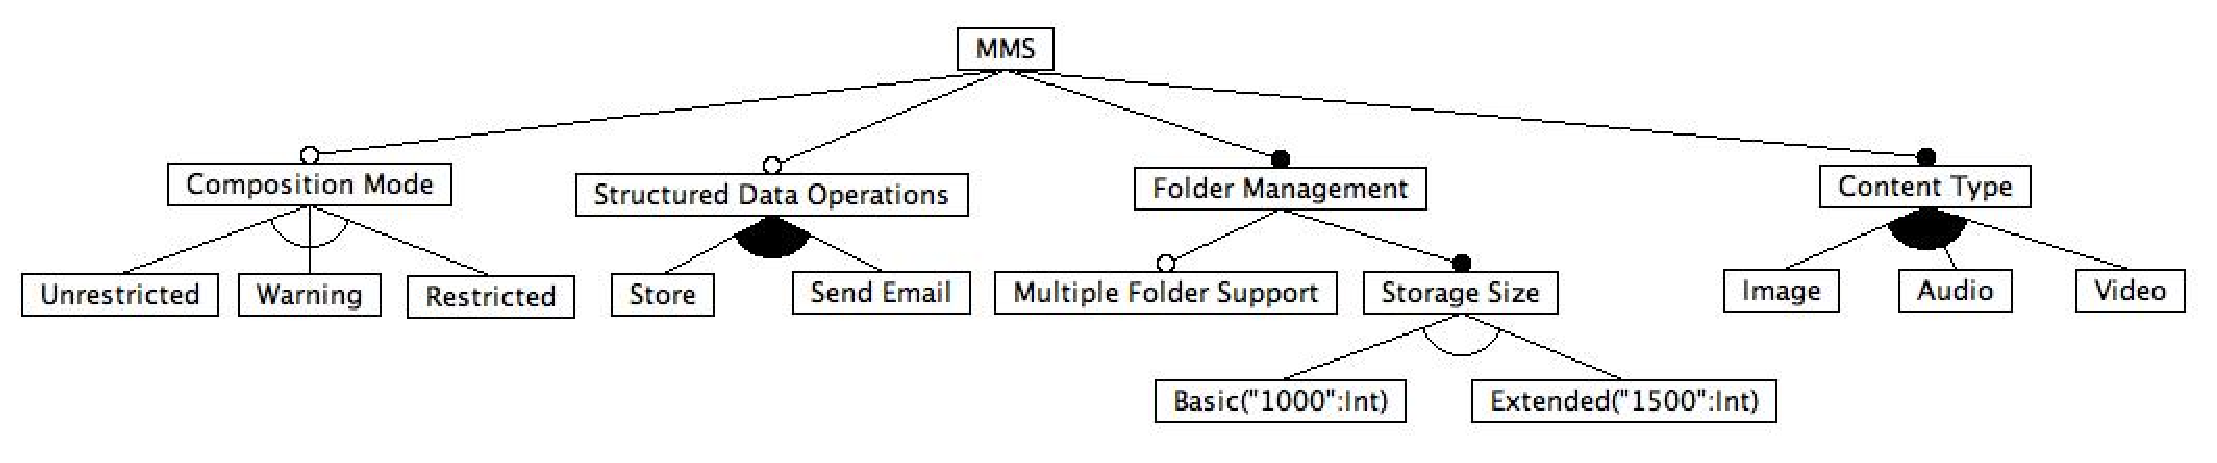
\epsfig{file=images/feature-model-01.eps,scale=0.45}
\caption{MMS feature model}
\label{mms-feature-model}
\end{figure*}

For simplicity, let us assume that three products (Table~\ref{tab:initial-products}) were defined in the SPL. 
This is required because some tags in PLUC technique, which will be explained later, are computed based on the specific members 
of the product line. 

\begin{table}[hb]
\centering
\caption{Initial set of products}
\label{tab:initial-products}
\begin{small}
\begin{tabular}{|c|l|} \hline
Product & Feature Configuration \\ \hline
P1  & Content Type (Image) {\bf and} \\ 
      & Folder Management (Size (1000))\\ \hline
P2  & Content Type (Image, Audio, Video) {\bf and} \\ 
      & Structured Data Operations (Store) {\bf and} \\ 
      & Folder Management (Size (1000))  \\ \hline
P3  & Content Type (Image, Audio, Video) {\bf and} \\ 
      & Structured Data Operations (Store, Send Email) {\bf and}\\
      & Composition Mode {\bf and} \\
      & Folder Management (Size (1500), Multiple Folder)  \\ \hline 
\end{tabular}
\end{small}
\end{table}

The first configuration corresponds to a simple product, with support for image content only, maximum number of messages equals to one thousand, and no support for structured data operations and DRM composition mode. The second one has support for all kinds of contents, the same maximum number of messages (one thousand), and full support for structured data operations. The later one also has support for all kinds of contents, extended storage size (maximum number of messages equals to one thousand and five hundreds), full support for structured data operations, support for DRM composition mode and Multiple Folders. One of the increments for the MMS product line, discussed in Section~\ref{evolution-analysis}, corresponds to the definition of new products. 

Next, we will present the specification of the \emph{Crate and Send a Message} use case using PLUC and PLUSS techniques. The necessary description of both notations is also presented.  

\subsection{Scenario specification in PLUC}
\label{sub:pluc}

Product Line Use Cases (PLUC) is a technique proposed for representing SPL requirements~\cite{bertolino-esec-2003}.  For instance, Figure~\ref{fig:pluc-01} presents 
the PLUC specification of \emph{Create and Send a Message}. This artifact is responsible for describing the behavior related to create and send a message and 
all of its extensions. In Figure~\ref{fig:pluc-01}, only two extensions are presented: \emph{Include a Multimedia Content} and 
\emph{Include a DRM Restricted Content in Restricted Mode}. Due to size constraints, other scenarios are not depicted in Figure~\ref{fig:pluc-01}. 


PLUC introduces special tags for representing variabilities in use case scenarios.  For example, Tag {\bf [VP3]}, in Step 6.a1 of Figure~\ref{fig:pluc-01}, denotes a variation 
point that abstracts over the supported content types. For each variation point used in scenario specification, one tag must be defined.
The actual value of each tag is specified in the \emph{Variation Points} section and depends on each product specification. It is important to notice 
that SPL members are also described using the same tag notation (see the {\bf VP1} tag in Figure~\ref{fig:pluc-01}). 

In PLUC, there is no specific artifact used to relate product configurations to feature models. In the current example, 
three products (Product 1, Product 2, and Product 3) are defined based on the initial set of products (Table~\ref{tab:initial-products}). Since the values of alternative and optional variation 
points are computed based on such products (as can be seen from the case-of clause in Figure~\ref{fig:pluc-01}), instead of specific features, the inclusion of a new member in the product line might require a deep review of 
all variation points. Moreover, since the variation points and the product definitions are spread among several PLUC artifacts, preserving the SPL consistency is 
hard and time consuming. A systematic analysis of such properties is described in Section~\ref{evaluation} 

\begin{figure}[t]
\begin{center}
\begin{tiny}
\fbox{
  \texttt{
  \begin{tabular}{l}
  {\bf Create and Send a Message} \\
  {\bf Goal:} Create and send a multimedia message \\
  {\bf Primary actor:} Subscriber \\ \\
  {\bf Main Flow:}  The message box has not reached {\bf [VP2]} messages. \\
  1. The subscriber starts the message center application \\
  2. The message center application is started \\
  3. The subscriber selects Create New MMS option \\
  4. The create a new MMS form is displayed \\
  5. The subscriber fills in the message body \\
  6. The subscriber selects the send message option \\
  7. The recipient form is displayed \\
  8. The subscriber fills in the recipient field \\ 
  9. The recipient field is filled \\
10. The subscriber selects the confirm option \\
11. The message is sent to the recipient \\
12. The message is saved in the sent folder \\
13. The send message transient is displayed \\
14. The application returns to message center \\ \\
{\bf Extensions} \\ \\
{\bf 6 Include a multimedia content} \\
6a.1.The subscriber selects the include a {\bf [VP3]} content option \\
6a.2.The list of all {\bf [VP3]} available resources is displayed \\
6a.3.The subscriber selects one specific resource \\
6a.4.The selected resource is attached to the multimedia message \\
6a.5.The application returns to step 6 \\ \\
{\bf 6 Include a DRM restricted content in Restricted Mode} \\
6b.1.The subscriber selects the include a {\bf [VP3]} content option \\
6b.2.The list of all [VP3] available resources is displayed \\
6b.3.The subscriber selects one DRM restricted resource \\
6b.4.The system reports the DRM restriction \\
6b.5.The application returns to step 6 \\ \\
{\bf Other extensions should be described here} \\ \\
{\bf Variation points: } \\ \\
   {\bf VP1: Alternative} \\
      0 : Product 1 \\
      1 : Product 2 \\
      2 : Product 3 \\
   {\bf VP2: Parametric} \\
      {\bf case VP1 of} \\
       0 : 1000 \\
       1 : 1000 \\
       2 : 1500 \\
   {\bf VP3: Parametric} \\
      {\bf case VP1 of} \\
       0 : (Image) \\
       1 : (Image, Audio, Video) \\
       2 : (Image, Audio, Video) \\    
   \end{tabular}
  } }
\end{tiny}
\end{center}
\caption{\emph{Create and Send a Message} in PLUC}
\label{fig:pluc-01}

\end{figure}

\subsection{Scenario specification in PLUSS}
\label{sub:pluss}

PLUSS (Product Line Use case modeling for Systems and Software engineering) is the other technique used in our comparative analysis. This approach presents a better separation 
between variability management and scenario specification, since product definition is not tangled within use cases, 
and the domain values of parameters (similar to PLUC tags) are related to alternative features and are 
not embedded in specifications~\cite{eriksson-splc-2005}. 

However, according to PLUSS meta-model~\cite{eriksson-splc-2005}, there is no specific artifact (such as configuration knowledge~\cite{czarnecki-book, phol-spl-book}) used for relating  features to optional use cases, scenarios and steps. Another characteristic of PLUSS is that all variant steps of a scenario specification are defined in the same flow of events. 
For example, the third flow presented in Figure~\ref{fig:pluss-01} describes the behavior related to the attachment of 
a DRM restricted content when a product is configured in both \emph{restricted} or \emph{warning} mode. Steps 2(a) and 2(b) are 
never performed together. They are alternative steps: Step 2(a) will be performed only if the feature \emph{Restricted composition 
mode} is selected; otherwise Step 2(b) will be performed. Additionally, Step 3 is optional, and will be performed only if the feature 
\emph{Warning composition mode} is selected. Therefore, based on PLUSS notation, features must be directly related to the use case 
model. 

In the current example, it is necessary to annotated the PLUSS feature model in order to represent that the 
\emph{Storage Size} feature is related to the {\bf Size} parameter; the \emph{Content Type} feature is related to the {\bf ContentType} parameter; the \emph{Restricted composition mode} feature is 
related to the Step 2(a) of second extension; and the \emph{Warning composition mode} feature is 
related to steps 2(b) and 3 of the second extension. Finally, notice that the behavior described in the second 
extension of Figure~\ref{fig:pluss-01} might be required in other use cases, like \emph{Selecting a Message to Forward} - 
since it is possible to attach a multimedia content while forwarding a message. Hence, a feature behavior can be spread 
among several use cases, resulting in maintainability issues: introducing a new product 
variant might require changes in several artifacts.

\begin{figure}[h]
\begin{center}
\begin{tiny}
  \texttt{
  \begin{tabular}{l}
  {\bf Create and Send a Message}  \\
  {\bf Goal:} Create and send a multimedia message  \\
  {\bf Primary actor:} Subscriber \\ 
  {\bf Main Flow:}  The message box has not reached {\bf [SIZE]} messages. \\ \\
  \end{tabular}
  \begin{tabular}{|p{0.2in}|p{1.4in}|p{1.4in}|}
  \hline 
  id & Actor Action & System Response \\ \hline 
  1  & Starts the message center application & The message center application is started \\ \hline
  2  & Selects Create New MMS option & The create a new MMS form is displayed \\ \hline
  3  & Fills in the message body and selects the send message option & The recipient form is displayed \\ \hline
  4  & Fills in the recipient field & The recipient field is filled \\ \hline
  5  & Selects the confirm option & The message is sent to the recipient and saved in the sent folder. The application returns to message center \\ \hline
 \end{tabular}
 %First extension flow in PLUSS example 
 \begin{tabular}{l}
  \\
 {\bf Extension Flow:}  Include a multimedia content \\ \\
 \end{tabular}
  \begin{tabular}{|p{0.2in}|p{1.4in}|p{1.4in}|}
  \hline 
  Id & Actor Action & System Response \\ \hline 
  1  & In the third step, the subscriber selects the include a {\bf [ContentType]} content option & The list of all {\bf [ContentType]} available resources is displayed \\ \hline
  2 & Selects one specific resource & The selected resource is attached to the multimedia message and the application returns to step 6 \\ \hline
  \end{tabular} 
 %Second extension flow in PLUSS example  
  \begin{tabular}{l} 
     \\
    {\bf Extension Flow:}  Include a DRM restricted content \\ \\
  \end{tabular}
  \begin{tabular}{|p{0.2in}|p{1.4in}|p{1.4in}|}
   \hline
   id & Actor Action & System Response \\ \hline 
   1 & Selects the include a {\bf [ContentType]} content option & The list of all {\bf [ContentType]} available resources is displayed \\ \hline
   2(a) & Selects one DRM restricted resource & The system reports the DRM restriction: the subscriber can not attach the resource \\ \hline
   2(b) & Selects one DRM restricted resource & The system asks the subscriber if he (she) wants to send a DRM restricted content \\ \hline
   (3)  & Confirms the attachment operation     & The selected resource is attached to the multimedia message \\ \hline
  \end{tabular} 
 } 
\end{tiny}
\end{center}
\caption{\emph{Create and Send a Message} in PLUSS}
\label{fig:pluss-01}

\end{figure}

In what follows, we present a systematic evaluation of our crosscutting approach by comparing it with the techniques just presented. As 
explained early, we performed three kinds of analysis in this evaluation: DSM analysis; quantitative analysis using modularity and 
complexity metrics; and SPL evolutionary analysis, where several increments to the MMS product line are considered.

%===============================================
% Evaluation
%===============================================
\section{Evaluation}
\label{evaluation}

As briefly discussed in Section~\ref{sub:pluc} and Section~\ref{sub:pluss}, both PLUC and PLUSS approaches do not present a
clear separation between variability management concern and scenario specification. This occurs because variants in PLUC 
are embedded in use case specifications; and, although variants in PLUSS are not tangled within use cases, such technique 
requires a direct relation from features to use cases. As a result of this kind of dependency, its is difficult to evolve both 
representations independently. 

In this section, 
we present a comparative analysis based on Design Structure Matrices (DSMs)~\cite{clark-design-rules-book}. 
DSMs is an interesting and simple tool for visualizing dependences between design decisions. Such decisions are distributed in both rows and columns of a matrix. We can identify which input data is required (a dependency) by a design task by observing which columns are marked in its corresponding row. However, DSMs do not offer support for 
quantifying relevant properties of scenario variability management. Therefore, we also present an evaluation based on modularity and 
complexity metrics. Finally, in order to increase the confidence of our previously evaluations, we analyze how the compared approaches support 
some common SPL increments, such as introducing a new feature variant and introducing a new product configuration. 

\subsection{DSMs analysis}
\label{dsm-analysis}

In this work, we apply DSMs to visualize 
design dependences in two levels: the first one presents a high level view of dependences between variability
management (feature model, SPL instances and configuration model) and use cases; the second
one presents how features are spread among use cases. 

Observing the high level view of dependences in PLUC (Figure~\ref{dsm:hl-pluc}),  
we can realize that such technique results in cyclical dependences between use cases and variability
management. First, use cases refer to tags that are computed based on features and on specific 
SPL instances (dependences illustrated in line 4 with columns 1, 2, and 3). On the other hand, the relationship between 
features and artifacts and the definition of SPL instances are embedded in the use cases (dependences illustrated in lines 1, 2, 
and 3 with column 4). 

This is an example of a non-modular design, because, in PLUC,
the \emph{Create and Send a Message} use case (Figure~\ref{fig:pluc-01})
specifies the space variability for the \emph{Message Folder Size} and the \emph{Supported Content
Types} features. However, the same information is presented in the Receive a Message use case.
Additionally, the SPL valid instances (products) and its configurations are spread among
several use cases. These dependences result in several modularity issues, being difficult for: a) documenting variability
management and use case decisions in parallel; and b) evolving both representations independently.

\begin{figure}[hb]
\centering
\begin{small}
\begin{tabular}{llllll} \hline
& & 1 & 2 & 3 & 4 \\ \hline
1 & Feature model 		& 	& 	& 	& x \\ 
2 & SPL instances 		& x 	& 	& 	& x \\
3 & Configuration model 	& x 	& x 	& 	& x \\
4 & Use case model 	& x 	& x 	& x 	& \\ \hline
\end{tabular}
\end{small}
\caption{High level view of dependences in PLUC}
\label{dsm:hl-pluc}
\end{figure}

PLUSS partially solves (see Figure~\ref{dsm:hl-pluss}) the cyclical dependences just presented, since SPL instances and feature variants are 
not embedded in use cases. However,  there is a cyclical dependency between the feature model and the configuration knowledge, since there is no independent artifact used to relate features to use cases, Additionally, it is not possible to 
independently evolve parameters in use case specification and their domain values defined in feature models 
(resulting in the cyclical dependency between use cases and features).

\begin{figure}[h]
\centering
\begin{small}
\begin{tabular}{llllll} \hline
& & 1 & 2 & 3 & 4 \\ \hline
1 & Feature model 		& 	& 	& x   & x \\ 
2 & SPL instances 		& x 	& 	& 	&   \\
3 & Configuration model 	& x 	&  	& 	& x \\
4 & Use case model 	& x 	&  	&  	& \\ \hline
\end{tabular}
\end{small}
\caption{High level view of dependences in PLUSS}
\label{dsm:hl-pluss}
\end{figure}

Applying our approach results in a better separation (Figure~\ref{dsm:hl-cc}) between
variability management and use cases, since the relationships between them are specified in the
configuration knowledge (they are not established in the feature model, as in PLUSS). 
Additionally, in our approach, the domain values of use
case parameters are related to feature models using a map (or environment).

As explained before, in PLUSS, it is necessary to introduce some annotations in the feature model in 
order to define the domain values of a scenario parameter. On the other hand, in our approach, we introduced 
a third artifact (map or environment) responsible for this kind of relationship. Such map is composed by pairs 
\emph{Parameter name} x \emph{Feature id}. For the parameters presented in the running example, we need 
a mapping with the entries: 

\begin{center}
\small{
$\{<Size, StorageSize>, <ContentType, ContentType>\}$
}
\end{center}

In this way the name of features can 
change without breaking the use cases (only the environment should be
updated). Because use cases do not have explicit references to SPL instances and
configurations, introducing new features or SPL instances do not change the use case model.

\begin{figure}[h]
\centering
\begin{small}
\begin{tabular}{lllllll} \hline
& & 1 & 2 & 3 & 4 & 5 \\ \hline
1 & Feature model 		& 	& 	&      &  	&  	\\ 
2 & SPL instances 		& x 	& 	& 	&   	& 	\\
3 & Configuration model 	& x 	&  	& 	&  	& x	\\
4 & Environment		& x	&	&	&	&  	\\
5 & Use case model 	&  	&  	&  	&  x	& 	\\ \hline
\end{tabular}
\end{small}
\caption{High level view of dependences in crosscutting approach}
\label{dsm:hl-cc}
\end{figure}   

In the context of this work, DSMs were also applied for representing 
the spread of features into use cases. Such representation 
was very useful for computing the metric \emph{Feature Diffusion Over 
Use Cases}~\cite{garcia-taosd-2005} (explained in Section~\ref{quantitative-analysis}).  
Due to space constraints,  we do not present the PLUSS DSM in this level of details. 

We can observe in the DSM of Figure~\ref{dsm:ll-pluc} that, in PLUC, features are often spread among several 
use cases. For example, feature \emph{Composition Mode} is relevant in the context of four use cases
(labeled as the design parameters 5 to 8). Other interesting characteristic, which we can
observe in the Figure~\ref{dsm:ll-pluc}, is that there is no dependences between use cases, since each use
case describes all of its extension points. However, it is not possible to specify two use
cases independently, since there is cyclical dependences between use cases and features
and these features can be spread into several use cases.

\begin{figure}[t]
\centering
\begin{scriptsize}
\begin{tabular}{llllllllll} \hline
								& 1 	& 2 	& 3 & 4 	& 5 	& 6 	& 7 	& 8 	& 9 	\\ \hline
1 Composition mode 				& 	& 	& 	& 	& x	& x	& x	& x	& 	\\
2 Structured data operations	 		& 	& 	& 	& 	& 	& x	& x	& 	& 	\\
3 Folder management 				& 	& 	& 	& 	& x	& x	& 	& 	& x	\\
4 Content type						& 	& 	& 	& 	& x	& x	& 	& 	& 	\\ \hline
5 Create and send a message 			& x	& 	& x	& x	& 	& 	& 	& 	& 	\\
6 Receive a message 				& x	& x	& x	& x	& 	&	& 	& 	& 	\\
7 Select and display a message 		& x	& x	& 	& 	& 	& 	& 	& 	& 	\\
8 Configure composition mode 		& x	& 	& 	& 	& 	& 	& 	& 	& 	\\
9 Manage user defined folders 		& 	& 	& x	& 	& 	& 	& 	& 	& 	\\ \hline
\end{tabular}
\end{scriptsize}
\caption{Dependences between features and use cases in PLUC}
\label{dsm:ll-pluc}
\end{figure}   

In our approach, since one scenario can refer to steps specified in
another use cases (either using \emph{step ids} or \emph{annotations}), there are several 
dependences between use
cases. For example, in Figure~\ref{dsm:ll-cc}, \emph{Structured Data Operation} 
use case depends on \emph{Select and Display a Message} and on \emph{Receive a Message} use cases. 
However, features do not depend on use cases anymore (the variability space is not represented in use
cases), there is no cyclical dependences, and use cases are more concise (although the number
of use cases is greater than in PLUC). Use case conciseness can be observed by the number of
features that are not related to the primary goal of the use case but that are tangled within its
specification. Two new use cases were created: \emph{Forward a Message}, that allows the reuse related 
to forward an existing message; and \emph{Structured Data
Operations}, responsible for modularizing all specification related to the structured data operation
concern.

\begin{figure}[h]
\centering
\begin{scriptsize}
\begin{tabular}{llllllllll} \hline
								& 1 	& 2 	& 3 & 4 	& 5 	& 6 	& 7 	& 8 	& 9 	 \\ \hline
1 Composition mode 				& 	& 	& 	& 	& 	& 	& 	& 	& 		\\
2 Structured data operations	 		& 	& 	& 	& 	& 	& 	& 	& 	& 	\\
3 Folder management 				& 	& 	& 	& 	& 	& 	& 	& 	& 	\\
4 Content type						& 	& 	& 	& 	& 	& 	& 	& 	& 	\\ \hline
5 Create and send a message 			& 	& 	& x	& x	& 	& 	& 	& 	& 	\\
6 Receive a message 				& 	& 	& x	& x	& 	&	& 	& 	& 	\\
7 Select and display a message 		& 	& 	& 	& x	& 	& 	& 	& 	& 	\\
8 Configure composition mode 		& x	& 	& 	& 	& 	& 	& 	& 	& 	\\
9 Manage user defined folders 		& 	& 	& x	& 	& 	& 	& 	& 	& 	\\ 
10 Forward a message		 		& 	& 	& 	& 	& 	& x	& x	& 	& 	\\ 
11 Structured data operation	 		& 	& x	& 	& 	& 	& x	& x	& 	& 	\\ \hline 
\end{tabular}
\end{scriptsize}
\caption{Dependences between features and use cases in the crosscutting approach}
\label{dsm:ll-cc}
\end{figure}   

\subsection{Quantitative analysis}
\label{quantitative-analysis}

Based on the scenario specifications 
and on the DSM analysis (Section~\ref{dsm-analysis}), we derived several metrics for quantifying 
feature modularity and use case model complexity (related to the size of specifications). Adapted 
from~\cite{greenwood-ecoop-2007}, the proposed modularity metrics quantify two types of 
relations involving features and use cases. First, \emph{Feature Diffusion over Use Cases} (FDU)
is used for quantifying how many use cases are affected by a specific feature. For instance, in PLUC we 
can realize (Figure~\ref{dsm:ll-pluc}) that \emph{Composition Mode} feature affects \emph{Create and Send a Message}, 
\emph{Receive a Message}, \emph{Select and Display a Message} and \emph{Configure Composition Mode} use cases. So, the 
corresponding FDU value is equal to four. On the other hand, \emph{Number of Features per Use Case} (NFU)
is used for quantifying how many features are tangled within a specific use case. We assume that each use 
case should be interested in its primary goal, although several features might be related to the primary goal of a use case.
For example, \emph{Content Type} and \emph{Storage Size} features are part of the primary goal of \emph{Create and Send a
Message} use case. However, \emph{Composition Mode} and \emph{Structured Data Operations} do not compose
its primary goal - actually, a specific product can be assembled without such features. 
Therefore, NFU value for \emph{Create and Send a Message} PLUC is three. Moreover, 
we applied the metric \emph{Feature Diffusion over Scenarios} (FDS) in order 
to quantify how many internal use case members (scenarios) are necessary for the materialization of a specific feature.

Two metrics related to complexity were applied in this work. The first one, vocabulary size,
quantifies the number of use cases ($VS_{U}$) and scenarios ($VS_{S}$) required by each of evaluated
approaches. The second one, \emph{Steps of Specification} (SS), is related to the size of each 
scenario and identifies how many pairs \emph{User action} x \emph{System response} compose a specific scenario. 

Additionally, we also relate modularity to complexity by applying \emph{Features and Steps of Specification} (FSS), which 
counts the number of steps of specification whose main purpose is to describe the behavior of a feature. 
Table~\ref{tab:metrics} summarizes the evaluation of these metrics based on the case study.

\begin{table}[hb]
\centering
\caption{Modularity and complexity metrics}
\label{tab:metrics}
\begin{tabular}{lccc} \hline
					& PLUC 	& PLUSS 	& Crosscutting	\\ \hline
Mean value of FDU 		& 3.5	& 3.5	& 2		\\
Mean value of FDS 		& 6.25	& 5		& 4.25	\\
Mean value of NFU 		& 2		& 2		& 1		\\
Mean value of FSS 		&12		& 11		& 10.25	\\ 
VSU 					& 5		& 5		& 7		\\
VSS 					& 27		& 24		& 23		\\
SS 					& 75		& 64		& 56		\\	\hline
\end{tabular}
\end{table}

In Table~\ref{tab:metrics} we present the average value 
of some metrics, such as the mean value of \emph{Feature Diffusion over Use Cases} (FDU). Therefore, on the average, the running 
example points that that each feature in PLUC is tangled within 3.5 use cases. Notice that, 
since PLUC and PLUSS do not allow a scenario to crosscut other scenarios in different use cases, it is difficult to modularize 
features into a single use cases. The result is that, when comparing to the crosscutting approach, features are more 
diffused (FDU metric) and use cases are less concise (NFU) in these approaches. 
The crosscutting approach, in contrast, allows the composition of scenarios through \emph{from steps} and \emph{to steps} clauses. 
Such mechanism, although more expressive and formal, is similar to use case extensions~\cite{jacobson-oose, jacobson-reuse-book, jacobson-aosd-book}.

Another point is that \emph{vocabulary size metrics} (such as VSU and VSS) are better in the crosscutting and PLUSS approaches for different reasons. First, the number of scenarios in PLUSS is lower than in PLUC because a scenario in PLUSS might be used for describing all related variants. For instance, \emph{Include a DRM Restricted Content} scenario of Figure~\ref{fig:pluss-01} describes the behavior for both \emph{Restricted} and \emph{Warning} modes. This facility is not supported in PLUC neither in crosscutting approach. However, in the crosscutting approach the vocabulary size is lower than in other approaches for the reason that a scenario might be modularized in such way that no duplications are required. For example, in PLUC and PLUSS approaches, since \emph{forward an incoming message} operation can be started from \emph{Receive a Message} and from \emph{Select and Display a Message} use cases, scenarios related to DRM constraints are duplicated. This problem can be avoided in our crosscutting approach by composing scenarios of different use cases.  
Also related to vocabulary size, the crosscutting approach presents more use cases than PLUC and PLUSS. However, 
the number and complexity of scenarios are lower. We discuss a bit more about these conclusions in Section~\ref{threats}. Next, 
we present the last evaluation we performed in this work.

\subsection{SPL evolution analysis}
\label{evolution-analysis}

This section aims to evaluate how the results of DSMs and quantitative analysis may be related 
to the flexibility, which is quantified by introducing some common SPL increments. The new version of MMS 
product line introduces a new \emph{structured data operation}, allowing a subscriber to make 
a call for a number embedded in a message;  introduce a new \emph{content type}, allowing a subscriber 
to attach emotion icons to messages; and defines a new product with the configuration presented by Table~\ref{tab:new-product}.

\begin{table}[hb]
\centering
\caption{New MMS product line member}
\label{tab:new-product}
\begin{small}
\begin{tabular}{|c|l|} \hline
Product & Feature Configuration \\ \hline
      & Content Type (Image, Audio, Emotion icons) {\bf and} \\ 
 P4 & Data Operations (Store, Send Email, Place a call) {\bf and}\\
      & Composition Mode {\bf and} \\
      & Folder Management (Size (1000), Multiple Folder)  \\ \hline 
\end{tabular}
\end{small}
\end{table}

Table~\ref{tab:incremental-results} summarizes the changes required by each SPL increment. We evaluate, for each technique, 
the impact of a given increment on  the following SPL artifacts: feature model (FM), configuration knowledge (CK), product configurations (PC), and use case model (UC). Specifically for the use case model, we present how many artifacts were impacted. For the other ones, we present only if the artifact was modified or not. 

The main conclusion is that defining domain values for parameters tangled within use cases requires a lot of effort to make simple 
changes, such as the inclusion of a new content type. In PLUC, this increment requires changes in all models. Additionally, each use 
case that refers to the content type must be updated.  Both PLUSS and crosscutting approaches, which use feature models to define 
the domain values of parameters, require only changes in feature models to introduce a new feature variant (a new content type, in 
this case). Based on the increments proposed, there is no significant difference between PLUSS and the crosscutting approach. However, since the behavior related to \emph{Strucure Data Operations} are modularized in one use case, in the
first increment, the number of affected use cases in the crosscutting approach is lower than in PLUSS. 

\begin{table*}[t]
\centering
\caption{Changes required in SPL increments}
\label{tab:incremental-results}
\begin{small}
\begin{tabular}{l|llll|llll|llll} \hline
& \multicolumn{4}{|c|}{PLUC} & \multicolumn{4}{|c|}{PLUSS}  & \multicolumn{4}{|c}{Crosscutting} \\
Increment 			& FM 	& CK   & PC & UC	& FM 	& CK & PC 	& UC 	& FM 	& CK & PC 	& UC  	\\ \hline
New data operation  	& x		& x	   & x    &	2	& x 		& x 	 & 		& 2		& x		& x	 & 		& 1		\\ 
New content type      	& x 		& x	   & x	    &	3	& x		&	 & 		& 0		& x		& 	 &		& 0		\\
New product definition 	& x 		& x	   & x	    &	3	& 		& 	 & x	 	& 0		& 		& 	 & x		& 0		\\ \hline
\end{tabular}
\end{small}
\end{table*}
  
\subsection{Threats to conclusion validity}
\label{threats}

We have chosen the MMS product line because it offers the opportunity of specifying different kinds 
of variability, such as \emph{optional use cases and scenarios}, \emph{parameterized scenarios} and 
\emph{crosscutting changes}. However, we concluded that some differences in the quantitative 
analysis might be observed after evaluating other product lines. For instance, besides some issues related 
to understandability, combining different variants in a single scenario might reduce significantly the  
specification's vocabulary size. This characteristic is only supported by the PLUSS approach. However, in 
the running example, only one feature was suitable for being specified using this technique.  

%Additionally, there are few examples available of PLUC and PLUSS use cases. Based on 
%such examples, we assumed that, in both techniques, one scenario can not crosscut scenarios in 
%other use cases. Using the \emph{from step} and \emph{to step} clauses (Section~\ref{scenario-variability}),
% such kind of crosscutting is possible in our approach. We have just 
%started contact with the authors of PLUC and PLUSS techniques in order to validate our 
%specifications using these techniques. However, the evaluation discussed in Section~\ref{evaluation} is
%still valid; once it can be used as a guide to perform other analysis and to report the benefits of the SoC between variability management 
%and SPL assets. 

\section{Related Work}
\label{related-work}

Several approaches have been proposed for representing 
scenario variability~\cite{jacobson-reuse-book, favaro-icsr-98, eriksson-splc-2005,bertolino-esec-2003}. However, in this 
paper we only compare our crosscutting approach with PLUC and 
PLUSS techniques. We choose these techniques because they encompass a broad range of SoC between 
variability management and scenario specification. PLUC presents the lowest level of 
modularity, since almost all information related to variability is described tangled within use cases. On the other hand, PLUSS 
partially reduces such coupling, by considering the importance of feature modeling.
 
However, still in PLUSS there are some dependences from feature to use cases that are avoided in our crosscutting approach. We 
achieve this level of modularity by introducing other artifacts that encapsulate relationships between features and use cases. 

Design Structure Matrices (DSMs) and crosscutting metrics have being applied for assessing modularity in \emph{aspect-oriented} 
systems~\cite{vlopes-aosd-2005, sullivan-fse-2005,garcia-taosd-2005, greenwood-ecoop-2007}. In this work, we also applied DSMs in the context of scenario variability management. Moreover, we customized a suite of metrics for quantifying feature diffusion and tangling over use cases. To our knowledge, our work is unique in applying both DSMs and crosscutting metrics for evaluating SoC in scenario variability.


%It is important to notice that the primary goal of existing works is to provide variation points in use case scenarios. Hence, the main 
%difference of our crosscutting approach  is that we introduced the intent of creating a better 
%separation between variability management and scenario specification. 

%Besides the discussion related to its paradoxical success~\cite{steimann-oopsla-2006}, 
%several works reported about the modularity benefits of AO systems. Some of this works 


\section{Concluding Remarks}
\label{concluding-remarks}

Variability management is a common challenge in software product line adoption. Although several 
works have been proposed for managing variabilities at scenario specification, existing works focus on 
representing variation points at use case documentation. In this paper we reported that we also need to 
introduce a modular perspective in this domain. On the reason that, if variability management is tangled within scenario 
specifications, it will be difficult to evolve both representations . Our analysis were based on customizations of recent techniques for software modularity assessments, such as \emph{Design Structure Matrices} and crosscutting concerns metrics. We showed that, in order to introduce common SPL increments, a clear separation between variability management and use case specifications is extremely valuable. As future work, we aim to evaluate other product lines and improve the presented metric suite. 

%
% The following two commands are all you need in the
% initial runs of your .tex file to
% produce the bibliography for the citations in your paper.
\bibliographystyle{abbrv}
\bibliography{rbonifacioEarlyAspects}  % sigproc.bib is the name of the Bibliography in this case
% You must have a proper ".bib" file
%  and remember to run:
% latex bibtex latex latex
% to resolve all references
%
% ACM needs 'a single self-contained file'!
%
%APPENDICES are optional
%\balancecolumns
\end{document}
